\chapter{Subgradients}
\label{chap:subgradients}

\section{Definition and properties}
\label{sec:subgradient_definition}

As we saw already in Chapters \ref{chap:convex_sets_functions} and
\ref{chap:optimization_basics}, derivatives play a key role in understanding the
properties of convex functions and convex optimization more broadly. But of
course, not all convex functions are differentiable. In this chapter, we will
develop a generalized notion of lower differentiability. % that will help us
%study and understand the behavior of essentially all convex functions.

For a function $f$ on $\R^d$, we say that $s \in \R^d$ is a \emph{subgradient} 
of $f$ at $x \in \dom(f)$ provided that
\index{subgradient}
\begin{equation}
\label{eq:subgradient}
f(y) \geq f(x) + s^\T (y-x), \quad \text{for all $y \in \dom(f)$}.
\end{equation}
This is analogous to the first-order characterization for convexity
\eqref{eq:first_order_characterization}, where $s$ playes the role of $\nabla
f(x)$: here, $s$ defines a linear map that passes through $f$ at $x$, and lies  
below $f$ everywhere. See Figure \ref{fig:subgradient} for an illustration. 

\begin{figure}[tb]
\centering
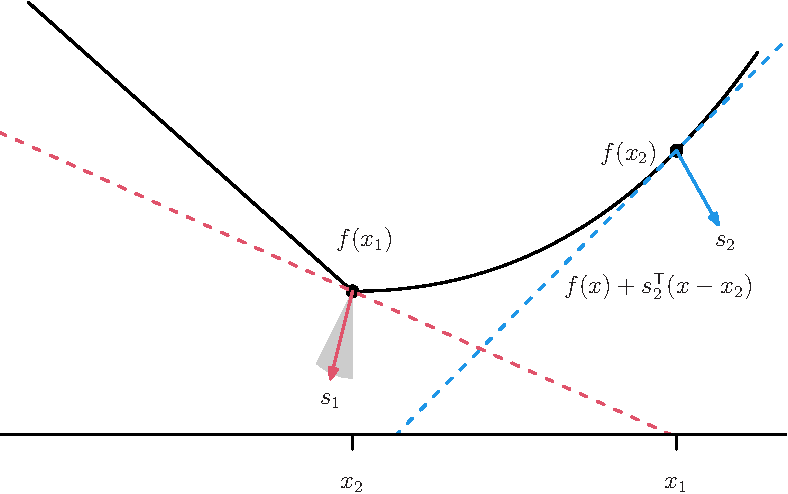
\includegraphics[width=0.7\textwidth]{fig/subgradient.pdf}
\caption{Two example subgradients $s_1$ and $s_2$ of a function $f$ at two
  points $x_1$ and $x_2$, respectively. Each $s_i$ defines a linear map 
  that passes through $x_i$ and lies below $f$ everywhere (that is, it defines a
  supporting hyperplane to $\epi(f)$ at $x_i$, whose normal is $(s_i,-1)$). At
  $x_2$, $f$ is differentiable, and $s_2 = \nabla f(x_2)$ is the only
  subgradient; at $x_1$ there are many possible subgradients (as illustrated
  by the gray wedge).}
\label{fig:subgradient}
\end{figure}

\index{subdifferential}
The set of all subgradients of $f$ at $x$ is called its \emph{subdifferential}
at $x$, which we denote by $\partial f(x)$. One can check that $\partial f(x)$
is always a closed convex set (regardless of whether $f$ itself is convex).  If
$\partial f(x)$ is nonempty, then $f$ is said to be \emph{subdifferentiable} at
$x$. Sometimes we will use a subscript on the subdifferential operator to
emphasize the variable under consideration. For example, when $f$ is a function 
of a block variable $(x,y)$, we use $\partial_x f(x,y)$ for the subdifferential
of the function $f(\cdot, y)$ at $x$, with its second argument fixed at $y$.

The notions defined above are apparently general, in that we have not assumed 
convexity of the function $f$ in question. However, as we will see in our 
discussion of some of the basic properties of subgradients and subdifferentials
below, these concepts are in fact intimately tied to convexity.   

\paragraph{Existence of subgradients.}

By rearranging the inequality in \eqref{eq:subgradient}, one finds that 
\index{subgradient!epigraph representation}
\[
s \in \partial f(x) \iff \text{$\epi(f)$ has a supporting hyperplane at
  $(x, f(x))$ with normal vector $(s, -1)$.}
\]
We see that the existence of a subgradient of $f$ at a point is linked to the
existence of a supporting hyperplane at a certain point of $\epi(f)$. Given the
existence of supporting hyperplanes for convex sets, it is reasonable to expect
that subgradients also exist in some generality for convex functions (whose
epigraphs are convex). The next result gives the details.

\index{subgradient!existence}
\begin{Theorem}
\label{thm:subgradient_existence}
A convex function $f$ is subdifferentiable at every point in $\relint(\dom(f))$,
the relative interior of its effective domain. In particular, this means that a
convex function that is finite on all of $\R^d$ is subdifferentiable at every
point.   

\setlength{\parindent}{\normalparindent}
Conversely, if $f : \R^d \to (-\infty, \infty]$ is closed, the set $\dom(f)$ is
convex, and $f$ is subdifferentiable on $\relint(\dom(f))$, then $f$ must be
convex.          
\end{Theorem}

As alluded to earlier, the first part of Theorem
\ref{thm:subgradient_existence}, on the existence of subgradients for a convex
function, is based on applying the supporting hyperplane theorem to the epigraph
representation of subgradients; the proof is outlined in Exercise
\ref{ex:subgradient_existence}. The second part, on subdifferentiability
implying convexity, is based on a converse supporting hyperplane theorem; see
Exercises \ref{ex:converse_supporting_hyperplane} and
\ref{ex:subdifferentiability_implies_convexity}. 

\paragraph{Uniqueness of subgradients.}

The subgradient of $f$ at a given point $x \in \dom(f)$ need not be unique, that
is, the subdifferential $\partial f(x)$ (when nonempty) need not be a
singleton. So, when it is unique at $x$, what can we say about $f$ at $x$,
vis-a-vis differentiability? The answer is nothing, in general (Exercise
\ref{ex:subgradient_nonuniqueness}). However, for convex $f$, the subgradient of
$f$ is unique at $x$ if and only it is differentiable at $x$. This result is
stated formally next; Exercise \ref{ex:subgradient_uniqueness} walks through its
proof. 

\index{subgradient!uniqueness}
\begin{Theorem}
\label{thm:subgradient_uniqueness}
Let $f$ be a convex function. If $f$ is differentiable at a point $x \in
\dom(f)$, then it has a unique subgradient $s = \nabla f(x)$ at $x$. Conversely,
if $f$ has a unique subgradient $s$ at $x$, then it is differentiable at $x$ and
$\nabla f(x) = s$.  
\end{Theorem} 

% Theorem 25.1 in Rockafellar (1970)

An interesting practical consequence of the last result is that we can infer the
differentiability of a convex function at a point (based on it having only one
subgradient), when it may be otherwise hard to see this from first
principles. This is the case in several of the next examples.

\medskip

\begin{Example}
\label{xa:norm_subgradients}
The following are examples of subgradients of common norms. For the first two
examples, the claims can be checked directly using the definition. The others
follow from Property \parref{par:subgradient_supremum} and the dual
representation of the norm in question. % and for these we refer to exercises
% that trace out the details.      

\begin{enumerate}[label=\alph*., ref=\alph*]
\item For $f(x) = |x|$, we have 
  \[
  \partial f(x) = \begin{cases}
  \{+1\} & x > 0 \\
  \{-1\} & x < 0 \\
  [-1,1] & x = 0
  \end{cases}.
  \]

\item \parlab{xa:l1_norm_subgradients}
  For $f(x) = \|x\|_1$, subgradients $s \in \partial f(x)$ are points of the
  form:  
  \index{l1 norm@$\ell_1$ norm!subgradients}
  \[
  s_i \in \begin{cases}
  \{+1\} & x_i > 0 \\
  \{-1\} & x_i < 0 \\
  [-1,1] & x_i = 0
  \end{cases}, \quad i=1,\ldots,d.
  \]
  We see that the $\ell_1$ norm is differentiable at each point $x$ that does
  not lie on any of the coordinate axes ($x_i \not=0$ for all 
  $i=1,\ldots,d$).  

\item \parlab{xa:lp_norm_subgradients}
  For $f(x) = \|x\|_p$, and $1 < p < \infty$, let $1 < q < \infty$ be such that
  $1/p + 1/q = 1$. Then for $x \not= 0$, we have (Exercise
  \ref{ex:lp_norm_subgradients} part a):   
  \index{lp norm@$\ell_p$ norm!subgradients}
  \[
  s_i = \sign(x_i) |x_i|^{p/q} \cdot \|x\|_p^{-p/q}, \quad i=1,\ldots,d 
  \]
  as the unique subgradient in $\partial f(x)$, and for $x=0$, we have $\partial
  f(0) = \{s : \|s\|_q \leq 1\}$. We see that the $\ell_p$ norm, $1 < p <
  \infty$, is differentiable at any $x \not= 0$. Note that for $p=2$ in
  particular, we have:
  \[
  \partial f(x) = \begin{cases}
  \{x / \|x\|_2\} & x \not= 0 \\
  \{s : \|s\|_2 \leq 1\} & x = 0
  \end{cases}.
  \]

\item \parlab{xa:linf_norm_subgradients} 
  For $f(x) = \|x\|_\infty$, subgradients $s \in \partial f(x)$ are points of
  the form (Exercise \ref{ex:lp_norm_subgradients} part b): 
  \index{linf norm@$\ell_\infty$ norm!subgradients}
  \[
  s_i \in \begin{cases}
  [0,1] & \hphantom{-} x_i = \|x\|_\infty \\   
  [-1,0] & -x_i = \|x\|_\infty \\
  \{0\} & \, |x_i| < \|x\|_\infty 
  \end{cases}, \quad i=1,\ldots,d,
  \]
  where $\|s\|_1 \leq 1$. We see that the $\ell_\infty$ norm is differentiable
  at any $x$ that has a unique maximum absolute coordinate.  

\item \parlab{xa:operator_norm_subgradients} 
  For $f(X) = \|X\|_{\op}$, the operator norm, we have (Exercise
  \ref{ex:operator_norm_subgradients}):  
  \index{operator norm!subgradients}
  \[
  \partial f(X) = \conv \{ u v^\T : \|u\|_2 \leq 1, \, \|v\|_2 \leq 1, \, u^\T X
  v =  \|X\|_{\op} \}.  
  \]
  In other words, subgradients are given by convex combinations of outer 
  products of top left and right singular vectors of $X$. If the top singular
  value of $X$ has multiplicity one, then this outer product is unique (there is
  only one top left and right singular vector, up to sign flips), and the
  operator norm is differentiable at $X$ with derivative $u v^\T$.         

\item \parlab{xa:trace_norm_subgradients}  
  For $f(X) = \|X\|_{\tr}$, the trace norm, letting $X = U \Sigma V^\T$ denote
  the SVD of $X$, we have (Exercise \ref{ex:trace_norm_subgradients}):   
  \index{trace norm!subgradients}
  \[
  \partial f(X) = \{ U V^\T + W: \|W\|_{\op} \leq 1, \, U^\T W = 0, \, W V = 0
  \}. 
  \]
  In other words, subgradients are given by adding to $U V^\T$ a matrix $W$ of
  at most unit operator norm that is orthogonal to the columns of $U$ and the
  rows of $V$. If $X$ has full column rank or full row rank ($X^\T X$ or $X
  X^\T$ is invertible), then only $W=0$ satisfies these constraints, and the
  trace norm is differentiable at $X$ with derivative $U V^\T$.    
\end{enumerate}
\end{Example}

\section{Subgradient calculus}

We describe rules that will be helpful in the calculation of subgradients. 

%(We note the similarity in functional operations covered here to those covered
%in Chapter \ref{sec:operations_preserving_convexity}.)  

\paragraph{Scaling.}

For any function $f$, $x \in \dom(f)$, and $a>0$, it holds that $(\partial a
f)(x) = a \partial f(x)$. This is also trivially valid for $a=0$, provided that
$\partial f(x) \not= \emptyset$.  

\paragraph{Sum.}
\parlab{par:subgradient_sum}

For any functions $f_1,\ldots,f_n$, their sum $F = f_1+\cdots+f_n$ satisfies,
for any $x \in \dom(F)$,  
\[
\partial F(x) \supseteq \partial f_1(x) + \cdots + \partial f_n(x),  
\]
where on the right we interpret $U + V = \{u + v : u \in U, \, v \in V\}$, the
set sum (Minkowski sum) of $U,V$. Moreover, if $f_1,\ldots,f_n$ are convex,
and $\cap_{i=1}^n \relint(\dom(f_i)) \not= \emptyset$, then for any $x \in
\dom(F)$,   
\[
\partial F(x) = \partial f_1(x) + \cdots + \partial f_n(x).
\]

% Theorem 23.8 in Rockafellar (1970)

\paragraph{Partial supremum.}
\parlab{par:subgradient_supremum}

Let $f$ be a function acting on a block variable $(x,z)$. If $f(\cdot,z)$ is
convex for each $z \in Z$, then the partial supremum \smash{$F = \sup_{z \in Z}
  f(\cdot,z)$} satisfies, for any $x \in \dom(F)$,
\index{partial supremum!subgradients}
\[
\partial F(x) \supseteq \closure\left( \conv\Bigg( \bigcup_{z \in \bar{Z}(x)} 
  \partial_x f(x, z) \Bigg)\right),  
\]
where \smash{$\bar{Z}(x) = \{z \in Z : f(x,z) = F(x)\}$}, the set of points at
which the supremum at $x$ is achieved. In other words, for any $z$ such that
$f(x,z)$ achieves the supremum, the subgradients of the function $f(\cdot, z)$
at $x$ are subgradients of $F$ at $x$, along with limits of convex combinations
of them. Moreover, if $\relint(\dom(F)) \not= \emptyset$, $Z$ is compact, $f$ is
continuous on $\relint(\dom(F)) \times Z$, and $f(\cdot,z)$ is \emph{closed}
and convex for each $z \in Z$, then         
\begin{equation}
\label{eq:danskin_bertsekas}
\partial F(x) = \conv\Bigg( \bigcup_{z  \in \bar{Z}(x)} \partial_x f(x, z)
\Bigg), 
\end{equation}
a result known as the \emph{Danskin-Bertsekas theorem}.  An important special
case corresponds to a finite set $Z$: if $f_i$, $i=1,\ldots,k$ are closed and
convex, then their pointwise maximum \smash{$F = \max_{i=1,\ldots,k} \, f_i$}   
satisfies \smash{$\partial F(x) =  \conv(\cup_{i : f_i(x) = F(x)} \, \partial
  f_i(x))$}, for any $x \in \dom(F)$.

\paragraph{Partial infimum.}
\parlab{par:subgradient_infimum}

Let $f$ be a function acting on a block variable $(x,z)$. If $f$ is convex and
$Z$ is a convex set, then the partial infimum \smash{$F = \inf_{z \in Z}
  f(\cdot,z)$} satisfies, for any $x \in \dom(F)$ such that $F(x) > -\infty$,  
where we now denote \smash{$\bar{Z}(x) = \{z \in Z : f(x,z) = F(z)\}$}, 
\index{partial infimum!subgradients}
\[
\partial F(x) \supseteq \closure\left( \conv\Bigg( \bigcup_{z \in \bar{Z}(x)} 
\{ s : (s, 0) \in \partial f(x, z) \} \Bigg)\right),  
\]

\paragraph{Linear composition.}
\parlab{par:subgradient_linear}

Let $f : \R^k \to (-\infty, \infty]$ be convex, and let $A \in \R^{k \times d}$,
$b \in \R^d$. Then the function $F$ defined as $F(x) = f(Ax+b)$ satisfies, for 
any $x \in \dom(F)$, 
\index{composition!subgradients}
\[
\partial F(x) \supseteq A^\T \partial f(Ax + b).
\]
Moreover, if $(\col(A) + b) \cap \relint(\dom(f)) \not= \emptyset$, then for any  
$x \in \dom(F)$,  
\[
\partial F(x) = A^\T \partial f(Ax + b).
\]

% Theorem 23.9 in Rockafellar (1970)

\paragraph{General composition.}
\parlab{par:subgradient_composition}

Let $f : \R^k \to (-\infty, \infty]$, $g : \R^d \to \R^k$, and denote their
composition by $F = f \circ g$, that is, $F(x) = f(g(x))$. If $f$ is convex and
nondecreasing in each argument, and each component function $g_i$,
$i=1,\ldots,k$ is convex, then  
\index{composition!subgradients}
\[
\partial F(x) \supseteq \{ r_1 s_1 + \cdots + r_k s_k : r = (r_1, \ldots, r_k)
\in \partial f(g(x)), \, s_i \in \partial g_i(x), \, i=1,\ldots,k \big\}.
\]
Note that the conditions here are no less general than those in Property
\parref{par:function_composition}, on the convexity of a composition; see
Exercise \ref{ex:function_composition} part b.

\medskip

\begin{Example}
The following examples can be checked using subgradient calculus rules.

\begin{enumerate}[label=\alph*.]
\item For $f(x) = h_C(X)$, the support function \eqref{eq:support_function} of a 
  compact set $C$, we have 
  \index{support function!subgradients}
  \[
  \partial h_C(x) = \bigg\{ y : y^\T x = \sup_{z \in C} \, z^\T x \bigg\},
  \]
  A norm $\|\cdot\|$ is in fact a support function, corresponding to the set
  $C = \{x : \|x\|_* \leq 1\}$. Here $\|\cdot\|_*$ is itself another norm that
  we call the dual norm of $\|\cdot\|$, and thus $C$ can be called the dual norm
  unit ball. The connection between $\|\cdot\|$ and $\|\cdot\|_*$ is detailed
  later, in Chapter \ref{sec:dual_norms}, when we cover duality; for now we
  simply observe that we can write  
  \index{dual norm}  
  \index{norm!ball}
  \begin{equation}
  \label{eq:norm_dual}
  \|x\| = \sup_{\|z\|_* \leq 1} \, z^\T x,
  \end{equation}
  and therefore by the Danskin-Bertsekas theorem \eqref{eq:danskin_bertsekas}, 
  \index{norm!subgradients}
  \begin{equation}
  \label{eq:norm_subgradients}
  \partial \|x\| = \{ y : \|y\|_* \leq 1, \, y^\T x = \|x\| \}.
  \end{equation}
  This can be used as a starting point to establish the results on subgradients
  of specific norms given in Example \ref{xa:norm_subgradients} (Exercises   
  \ref{ex:lp_norm_subgradients}--\ref{ex:trace_norm_subgradients}). 

\item For $f(x) = \|Ax\|$, where $A \in \R^{k \times d}$ and $\|\cdot\|$ is a
  norm, we have
  \[
  \partial f(x) = \{ A^\T y :  \|y\|_* \leq 1, \, y^\T A x = \|Ax\| \}.
  \]
  Here $\|\cdot\|_*$ the dual norm of $\|\cdot\|$, as in the last example.

\item For $f(x) = \inf_{z \in C} \|x - z\|_2$, where $C$ is closed and
  convex, suppose $x \notin C$. Letting $P_C$ denote the (Euclidean)
  projection operator onto $C$, which satisfies $\|x - P_C(x)\|_2 = f(x)$, we
  have  
  \begin{equation}
  \label{eq:set_distance_subgradients}
  \partial f(x) = \bigg\{ \frac{x - P_C(x)}{\|x - P_C(x)\|_2} \bigg\}. 
  \end{equation}
\end{enumerate}
\end{Example}

\section{Subgradient optimality condition}
\label{sec:subgradient_optimality}

Subgradients have an important connection to the minimization of a function. The 
following can be checked directly from the definition of a subgradient in
\eqref{eq:subgradient}: $f(x) \leq f(y)$ for all $y$ if and only if
\index{subgradient!optimality condition}
\begin{equation}
\label{eq:subgradient_optimality}
0 \in \partial f(x). 
\end{equation}
This is called the \emph{subgradient optimality condition} for $f$. Note that it 
generalizes the more familiar zero-gradient condition \eqref{eq:zero_gradient}
for differentiable convex $f$, since for differentiable convex $f$, the only
subgradient at $x$ is the gradient $\nabla f(x)$ (Theorem
\ref{thm:subgradient_uniqueness}). We will soon find the subgradient optimality
condition \eqref{eq:subgradient_optimality} very useful, when we discuss
proximal operators in the next chapter; we will also see it playing a prominent
role in numerous subsequent parts of this book.  

This can be extended to an optimality condition for the constrained problem,
\[
\minimize_x \quad f(x) \quad \st \quad x \in C.
\]
for a convex function $f$ and convex set $C$, where $\relint(\dom(f)) \cap
\relint(C) \not= \emptyset$.  We rewrite this problem in characteristic form    
\[
\minimize_x \quad f(x) + I_C(x),
\]
and observe that $x \in C$ is a solution if and only if zero is a subgradient
of the criterion at $x$, which (using convexity of $f$ and $I_C$, and the
subgradient rule for a sum in Property \parref{par:subgradient_sum}), can be
written as $0 \in \partial f(x) + \partial I_C(x)$, that is,
\[ 
-s \in I_C(x), \quad \text{for some $s \in \partial f(x)$}. 
\]
It remains to compute the subdifferential of $I_C$, the characteristic function
of the convex set $C$. A straightforward calculation reveals     
\index{characteristic function!subgradients} 
\index{normal cone}
\[
\partial I_C(x) = \cN_C(x) = \{ s : s^\T x \geq s^\T y, \, \text{for all $y \in
  C$}\}. 
\]
the normal cone to $C$ at $x$, and the second-to-last display, the (necessary 
and sufficient) subgradient optimality condition for a constrained convex
problem, becomes      
\begin{equation}
\label{eq:subgradient_optimality_constrained}
s^\T (y - x) \geq 0, \quad \text{for some $s \in \partial f(x)$ and all $y \in 
  C$},
\end{equation}
which nicely generalizes the first-order optimality condition
\eqref{eq:first_order_optimality} covered in Chapter
\ref{sec:properties_convex_problems}. 

\section{Subgradient monotonicity*}

The subdifferential of a function $f$ is a \emph{monotone operator}, which means
that it satisfies 
\index{subgradient!monotonicity}
\begin{equation}
\label{eq:subgradient_monotonicity}
(s_x - s_y)^\T (x - y) \geq 0, \quad \text{for all $x,y \in \dom(f)$, and 
  $s_x \in \partial f(x)$, $s_y \in \partial f(y)$}.    
\end{equation}
For given $x,y$, the inequality can be seen by simply adding together the two
conditions defining the subgradients, $f(y) \geq f(x) + s_x^\T (y-x)$ and $f(x)
\geq f(y) + s_y^\T (x-y)$, and rearranging. Note that this generalizes the
monotone gradient condition \eqref{eq:gradient_monotonicity} satisfied by a
differentiable convex function. 

It is natural to ask whether there is a converse to the subgradient monotonicity
condition. For gradients, recall, there is a converse result: if $f$ is
differentiable, and $(\nabla f(x) - \nabla (y))^\T (x-y) \geq 0$ for all $x,y$,
then $f$ is convex (Exercise \ref{ex:gradient_monotonicity}). However, for
subgradients we will need to be careful at the outset, in even just posing the
question precisely. For example, if $\partial f(x) = \emptyset$ for all $x$, as
would be the case for (say) differentiable and strictly concave $f$, then
\eqref{eq:subgradient_monotonicity} is vacuously true, but clearly $f$ is not
convex. On the other hand, if we assumed that subgradients exist on
$\relint(\dom(f))$, then $f$ would already be convex (provided $f$ is closed;
recall Theorem \ref{thm:subgradient_existence}).

A way to pose the converse question precisely is as follows. Given a set-valued
operator $T$, with $T(x) \subseteq \R^d$ for each $x \in \R^d$ (and possibly
$T(x) = \emptyset$ for some $x$), if 
\index{monotone operator}
\begin{equation}
\label{eq:T_monotonicity}
(s_x - s_y)^\T (x - y) \geq 0, \quad \text{for all $x,y$, and $s_x \in T(x)$,
  $s_y \in T(y)$}, 
\end{equation}
then does there exist a convex function $f$ for which $T \subseteq \partial f$?
This is a kind of \emph{embedding} problem: we are asking whether the graph of
$T$ embeds into the graph of the subdifferential $\partial f$ of some convex
function $f$; or equivalently, given a set of pairs $\{ (x_i, s_i) : i \in I \}$
(the graph of $T$, where $I$ is possibly infinite), we are seeking a convex
function $f$ that satisfies the relations 
\[
f(y) \geq f(x_i) + s_i^\T (y-x_i), \quad i \in I.
\] 

Interestingly, monotonicity of $T$, as in \eqref{eq:T_monotonicity}, is not
enough, but a suitable generalization of this condition is. To motivate this,
let $(x_i, s_i)$, $i=1,\ldots,n$ denote any $n$ points in the graph of $\partial
f$; that is, satisfying $s_i \in \partial f(x_i)$, $i=1,\ldots,n$. Writing
$x_{n+1}=x_1$ for convenience, adding together the $n$ subgradient inequalities  
\[
f(x_{i+1}) \geq f(x_i) \geq s_i^\T (x_{i+1} - x_i), \quad i=1,\ldots,n,
\]
and rearranging, gives 
\begin{equation}
\label{eq:T_monotonicity_n}
s_1^\T (x_2 - x_1) + s_2^\T (x_3 - x_2) + \cdots + s_{n-1}^\T (x_n -
x_{n-1}) + s_n^\T (x_1 - x_n) \leq 0.
\end{equation}
An operator $T$ that satisfies \eqref{eq:T_monotonicity_n} for all $n \geq 1$
and all $(x_i, s_i)$, $i=1,\ldots,n$ in its graph is said to be \emph{cyclically
monotone}. The argument just given shows that $\partial f$ is itself cyclically
monotone.
\index{monotone operator!cyclical}

The next result, which we call \emph{Rockafellar's embedding theorem}, gives a
complete characterization of subgradients and monotonicity.  

\index{Rockafellar's embedding theorem}
\index{monotone operator!maximal}
\begin{Theorem}
\label{thm:rockafellar_embedding}
Let $T$ be a set-valued operator, where $T(x) \subseteq \R^d$ for $x \in
\R^d$. There exists a convex function $f$ with $T \subseteq \partial f$ (which
means that $T(x) \subseteq \partial f(x)$ for all $x \in \R^d$) if and only if
$T$ is cyclically monotone. 

\setlength{\parindent}{\normalparindent}
Moreover, there exists a closed convex function with $T = \partial f$ if and
only if $T$ is maximal cyclically monotone (where maximal means that there is no
other cyclically monotone map $T'$ with $T \subseteq T'$). Finally, when it
exists, the solution $f$ (to the equation $T = \partial f$) is unique up to an
arbitrary additive constant.
\end{Theorem}

% Rockafellar (1966)

Note that the ``only if'' direction for the containment result $T \subseteq
\partial f$ in Theorem \ref{thm:rockafellar_embedding} was already established
in the motivating discussion before the theorem statement. For other parts of
the proof of Theorem \ref{thm:rockafellar_embedding}, see Exercise
\ref{ex:rockafellar_embedding}.

\section{Subgradients and growth*}

The gradient monotonicity characterization \eqref{eq:gradient_monotonicity} for
convexity played a key role in the proofs of Theorems
\ref{thm:lipschitz_smoothness} and \ref{thm:strong_convexity}, which provided 
various equivalent growth conditions, in the case of smooth functions. As we
just saw in the last section, subgradients have a monotonicity characterization
as well. With subgradients in place of gradients, the next result essentially
generalizes Theorem \ref{thm:strong_convexity}.     

\index{strong convexity}
\begin{Theorem}
\label{thm:strong_convexity_nonsmooth}
For closed convex $f : \R^d \to (-\infty, \infty]$ and $m>0$, consider the
statements:     
\begin{enumerate}[label=(\roman*)]
\item $\|s_x - s_y\|_2 \geq m \|x-y\|_2$, for all $x,y \in \dom(f)$ and 
  $s_x \in \partial f(x)$, $s_y \in \partial f(y)$;  
\item the function $f_m$ is convex, where $f_m(x) = f(x) - \frac{m}{2}
  \|x\|_2^2$;    
\item $f(y) \geq f(x) + s_x^\T (y-x) + \frac{m}{2} \|y-x\|_2^2$, for all $x,y
  \in \dom(f)$ and $s_x \in \partial f(x)$; 
\item $(s_x - s_y)^\T (x - y) \geq m\|x-y\|_2^2$, for all $x,y \in \dom(f)$ and
  $s_x \in \partial f(x)$, $s_y \in \partial f(y)$.  
\end{enumerate}
Then the following relations hold: 
\[
\text{(i)} \impliedby \text{(ii)} \iff \text{(iii)} \iff \text{(iv)}.
\]
\end{Theorem}

The proof of Theorem \ref{thm:strong_convexity_nonsmooth} is outlined in
Exercise \ref{ex:strong_convexity_nonsmooth}, divided in two main parts. The
first part shows that $\text{(ii)} \iff \text{(iii)} \implies \text{(iv)}
\implies \text{(i)}$, using arguments entirely analogous to those used for
Theorem \ref{thm:strong_convexity} (Exercise \ref{ex:lipschitz_smoothness}). The
second part proves $\text{(iv)} \implies \text{(ii)}$, using Rockafellar's
embedding theorem, and a projection argument that reduces consideration to
set-valued operators on $\R$ (where monotone and cyclically monotone operators
coincide). An alternative proof for $\text{(iv)} \implies \text{(ii)}$ can be
given using generalized subgradients; see the chapter notes for more details.

It is worth noting that an important consequence of Theorem
\ref{thm:strong_convexity_nonsmooth} is that it establishes strongly convex
functions are coercive. See Exercise \ref{ex:strong_convexity_coercive}.

Next we give one more simple but important growth result, on the boundedness of
subgradients over compact sets. We remark that part (ii) of the next theorem in
fact establishes that a convex function is locally Lipschitz, as claimed in part
(iii) of Theorem \ref{thm:smoothness_properties}.  

\index{subgradient!boundedness}
\index{Lipschitz continuity}
\begin{Theorem}
\label{thm:subgradient_boundedness}
Let $f$ be a convex function, and let $C \subseteq \interior(\dom(f))$ be 
compact. Then:
\begin{enumerate}[label=(\roman*)]
\item $\cup_{x \in C} \, \partial f(x)$ is nonempty and bounded;  
\item $f$ is Lipschitz continuous on $C$, meaning (recall)
  \[
  |f(x) - f(y)| \leq L \|x-y\|_2, \quad \text{for all $x,y \in C$},
  \]
  with Lipschitz constant \smash{$L = \sup_{s \in \cup_{x \in C} \partial f(x)}
    \|s\|_2$}. 
\end{enumerate}
Further, as a converse to (i), the condition $x \in \interior(\dom(f))$ is also 
necessary for $\partial f(x)$ to be nonempty and bounded.   
\end{Theorem}

% For example, Proposition 5.4.2 in Bertsekas (2009) for (i) and (ii), and
% Theorem 23.4 in Rockafellar (1970) for the last part

% Note: the last statement shows we cannot relax \interior(\dom(f)) to
% \relint(\dom(f)) here! Outside of \interior(\dom(f)), the subdifferential is
% not bounded. This in particular also means that we cannot relax
% \interior(\dom(f)) to \relint(\dom(f)) in statements (ii)--(iv) of Theorem  
% \ref{thm:smoothness_properties}, or at least doing so seems nontrivial. 

\section{Subgradients and geometry*}

Subgradients possess a deep connection to convex geometry. Recall based on the
discussion before and after Theorem \ref{thm:subgradient_existence} that their
existence is tied to the fact that a subgradient of a function defines a normal
vector to its epigraph. A related interpretation is as follows: if $s \in
\partial f(x)$, then we observe straight from the definition
\eqref{eq:subgradient} that
\[
f(y) \leq f(x) \implies s^\T x \geq s^\T y.
\]
In other words, $s$ defines the normal to a supporting hyperplane of a sublevel
set $\{y : f(y) \leq f(x)\}$ at $x$. As the normal cone to $\{y : f(y) \leq
f(x)\}$ at $x$ is, by definition, the collection of all such normal vectors, we
can also write this conclusion as   
\[
\partial f(x) \subseteq \cN_{\{y : f(y) \leq f(x)\}}(x).
\]
Interestingly, as the next result shows, the subgradients at $x$ not only lie in
the normal cone to the sublevel set at $x$, they also generate it. 

\index{subgradient!normal cone representation}
\begin{Theorem}
\label{thm:subgradient_normal}
Let $f$ be a convex function, and $x \in \relint(\dom(f))$ be a point at which
$f$ does not attain its infimum. Then 
\[
\cN_{\{y : f(y) \leq f(x)\}}(x) = \cone\big(\partial f(x)\big).
\]
\end{Theorem}

% For example, Theorem 23.7 in Rockafellar (1970). Removing the cl() because the
% subdifferential is closed convex bounded and does not contain the origin, so
% its convex hull should be closed. As in Corollary 9.6.1 of Rockafellar (1970)

Just like the subgradient optimality condition \eqref{eq:subgradient_optimality}
generalizes the zero-gradient condition \eqref{eq:zero_gradient} from classical
smooth analysis, we can view Theorem \ref{thm:subgradient_normal} as a
generalization of the classical result that the gradient vector $\nabla f$ lies 
orthogonal to tangent planes of level sets a smooth function $f$. See Figure
\ref{fig:subgradient_normal} for an illustration. 

\begin{figure}[tb]
\centering
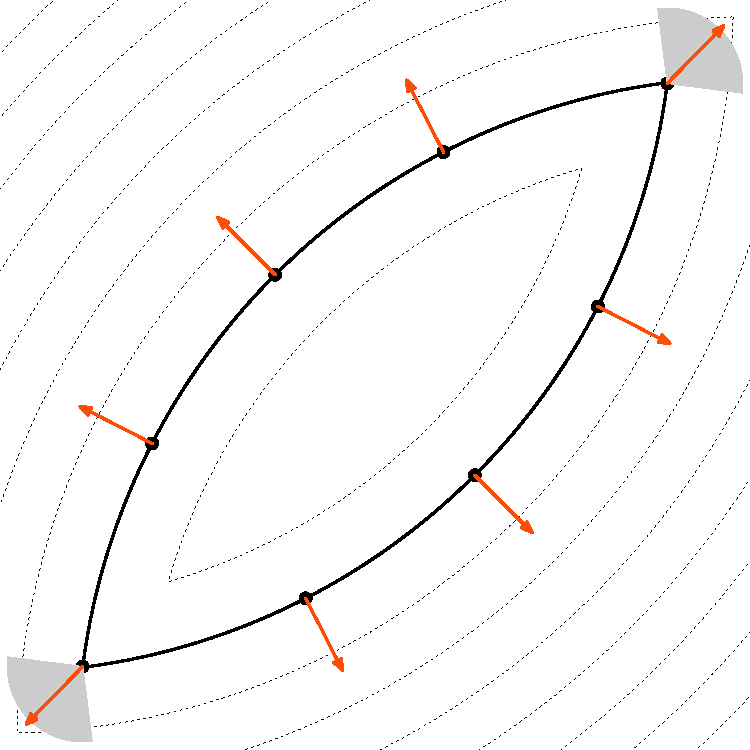
\includegraphics[width=0.525\textwidth]{fig/subgradient_normal.pdf}
\caption{Contours of a convex function $f$, with a particular level set of
  interest highlighted in solid black. At various points $x$ along the level
  set, subgradients of $f$ at $x$ are drawn, represented as normal vectors
  emanating from the level set at $x$. At two points along the level set, in the
  bottom left and top right, $f$ is not differentiable, and the subdifferentials
  are represented by gray wedges.}        
\label{fig:subgradient_normal}
\end{figure}

\index{subgradient!categorization}
Lastly, we discuss a categorization of points of subdifferentiability of $f$,
and we show how the geometric perspective provided in Theorem
\ref{thm:subgradient_normal} leads to an interesting conclusion about the number 
of points lying in the ``least smooth'' category, along any slice through the
graph of a convex function $f$. The categorization is as follows: when $k =
\dm(\spa(\partial f(x)))$, the dimension of the linear span $\partial f(x)$, we
say that $x$ is \emph{category $k$} point in the subdifferential $\partial
f(x)$. Thus, for convex $f$, at a point $x$ where $f$ does not attain its 
infimum: 
\begin{itemize}
\item $x$ is category 0 $\iff$ $f$ not subdifferentiable at $x$;
\item $x$ is category 1 $\iff$ $f$ is differentiable at $x$;
\item $x$ is category 2 $\iff$ $f$ has two linearly independent subgradients at 
  $x$, say $s_1$ and $s_2$, where $\spa\{s_1, s_2\} = \partial f(x)$; 
\item and so on, up through category $d$, where $\dom(f) \subseteq \R^d$. 
\end{itemize}
Points in category 1 can be thought of as the ``most smooth'', and points in
category $d$ as the ``least smooth'' (among categories 1 through $d$, excluding
0): for a point $x$ in category $d$ the normal cone to the sublevel set $\{y :
f(y) \leq f(x)\}$ at $x$ is $d$-dimensional, which means the sublevel set looks
``pointy'' at $x$, like a vertex on a polyhedron, or the bottom left and top
right points along the level set drawn in Figure \ref{fig:subgradient_normal}.   

We already know from Theorem \ref{thm:smoothness_properties} part (iii) that
categories 2 through $d$ are, altogether, ``rare'' compared to category 1: the
union of category 2 through $d$ points only make up a set of Lebesgue measure 
zero in $\interior(\dom(f))$. But in fact, we can say something much finer along
any slice through the graph of a convex function $f$: on any such slice, it
turns out that $f$ can only have a \emph{countable} number of points in category
$d$, the ``least  smooth'' category.  

\begin{Theorem}
\label{thm:subgradient_category_d}
Let $f$ be convex with $\dom(f) \subseteq \R^d$, and let $t \in \R$ be
arbitrary.  Then $f$ has a countable number of category $d$ subdifferentiable
points along the level set $\{x : f(x) = t\}$. 
\end{Theorem}

% For example, Proposition 11.6.2 in Berger (2004), Part I

The proof of Theorem \ref{thm:subgradient_category_d} is elementary, and it
rests critically on the normal cone formulation of subgradients in Theorem 
\ref{thm:subgradient_normal}. Essentially, it uses the normal cone relationship
(and convexity of the sublevel set) to argue that the interiors of 
conic hulls of category $d$ subdifferentials along the level set form a
collection of disjoint open sets in $\R^d$, and hence by classical arguments in 
analysis, there can be at most a countable number of them. See Exercise
\ref{ex:subgradient_category_d}.   

\SkipTocEntry\section*{Chapter Notes}

Jean Jacques Moreau and R. Tyrrell Rockafellar are widely considered to be the
``founding fathers'' of subdifferentiability, each having worked separately to 
develop the subject in the early 1960s. To learn more, beyond what is covered in
this chapter, a classic reference (and masterful treatment) is
\cite{rockafellar1970convex} (Chapters 23--25); we also recommend
\cite{hiriartUrruty2001fundamentals} (Chapter D) and \cite{bertsekas2009convex} 
(Chapter 5.4). The study of monotone operators is closely linked to the study of 
subgradients (and also to that of proximal operators, which will be covered in
the next chapter). Two nice books that develop this connection, from different
perspectives (analytic versus algorithmic) are \cite{bauschke2011convex,
  ryu2022large}.      

The Danskin-Bertsekas theorem is named after the extension given in Bertsekas'
Ph.D.\ thesis \cite{bertsekas1971control} of an earlier result by Danskin
\cite{danskin1967theory}. Even more can be said about the subdifferential of a
partial supremum of convex functions; see, for example,
\cite{hantoute2008subdifferential} for a recent overview and connections to
other subgradient calculus rules. Rockafellar's embedding theorem (which is not, 
as far as we know, a commonly used name for the result stated in this chapter)
is due to \cite{rockafellar1966characterization}.

Finally, we note that generalizations of the definition of a subgradient have
been developed for nonconvex functions, notably by Francis H.\ Clarke and
Rockafellar, in the 1980s. These definitions reduce to the usual notion of a
subgradient for convex functions, and also reduce the usual notion of a gradient
for differentiable (and possibly nonconvex) functions, but apply much more
broadly. Two authoritative references, each of which covers much more than just
generalized subgradients, are \cite{clarke1990optimization,
  rockafellar2009variational}. Generalized subgradients are not only critical
tools in nonsmooth and variational analysis, they can also be useful in
\emph{convex} analysis. For example, the generalized subgradient used in
variational analysis, as defined in \cite{rockafellar2009variational}, provides 
an alternative, short proof that $\text{(iv)} \implies \text{(ii)}$ in Theorem
\ref{thm:strong_convexity_nonsmooth}; see Exercise 12.59 in
\cite{rockafellar2009variational}.   

\clearpage

\begin{xcb}{Exercises}
\begin{enumerate}[label=\thechapter.\arabic*]
\settowidth{\leftmargini}{0.00.\hskip\labelsep}
\index{supporting hyperplane theorem!converse}
\item \label{ex:converse_supporting_hyperplane}
  This exercise proves the following converse to the supporting hyperplane
  theorem: if $C$ is a closed set, $\relint(C) \not= \emptyset$, and every $x_0
  \in \relbd(C)$ has a supporting hyperplane (there exists $a\not=0$ and $b$  
  such that $a^\T x_0 = b$ and $a^\T x \leq b$ for all $x \in C$), then $C$     
  must be convex.   

  We will assume, without a loss of generality, that $C$ is full-dimensional
  ($\aff(C) = \R^d$), so its relative interior and relative boundary are its
  interior and boundary, respectively. (Note: having proved this
  full-dimensional result, to accommodate the case when $\aff(C)$ is a proper
  subspace of $\R^d$, we can reparametrize to the affine subspace, and apply the
  result just proved to conclude that the set $D$---the reparametrization of $C$
  to the affine subspace---is convex in this coordinate system, and then simply
  view $C$ as an affine image of $D$ in order to conclude that $C$ itself is
  convex.)  

  Let $H$ be the intersection of all supporting halfspaces to $C$, 
  \[
  H = \bigcap_{x_0 \in \boundary(C)} \underbrace{\{ x :  a_{x_0}^\T x \leq
    b_{x_0} \}}_{H_{x_0}}, 
  \]
  where for each $x_0 \in \boundary(C)$, we write \smash{$a_{x_0}$} and
  \smash{$b_{x_0}$} for the normal vector and offset, respectively, that define
  the supporting hyperplane to $C$ at $x_0$. Note that $H$ is convex, and that
  $C \subseteq H$.    

\begin{enumerate}[label=\alph*.]
\item Fix $y \notin C$, and let $x \in \interior(C)$. Let
  \[
  t = \sup \{ s \geq 0 : x + s (y - x) \in C \}. 
  \]
  Prove that $s \in (0,1)$. (Hint: use that $x \in \interior(C)$, and the fact
  that $C^c = \R^d \setminus C$ is open.) Prove also that $t y \in
  \boundary(C)$. (Hint: use again the fact that $C$ is closed.) 

\item By inspecting the supporting hyperplane at $x_0 = t y$, argue that since
  $x \in H_{x_0}$, we must have \smash{$y \notin H_{x_0}$}, and thus $y \notin 
  H$. 

  \smallskip
  Since $y$ was arbitrary, note that we have shown $C^c \subseteq H^c$, that is,
  $H \subseteq C$, which together with the observation $C \subseteq H$, proves
  that $C = H$ and hence that $C$ is convex. 
\end{enumerate}

\index{subgradient!existence}
\item \label{ex:subdifferentiability_implies_convexity}
  We will now prove the second part of Theorem \ref{thm:subgradient_existence},  
  using the converse supporting hyperplane theorem from Exercise
  \ref{ex:converse_supporting_hyperplane}. Let $f$ satisfy the conditions of the 
  theorem: $f : \R^d \to (-\infty, \infty]$ is closed and has a subgradient and   
  every point in $\relint(\dom(f))$, where $\dom(f)$ is convex.

\begin{enumerate}[label=\alph*.]
\item Abbreviate $S = \relint(\dom(f))$. Prove that any point $(x,t)$ on the
  relative boundary of $\epi(f)$ can be written in one of two ``types'': 
  \begin{alignat*}{2}
  &\text{type I}: \quad &&x \in S, \; t = f(x), \\
  &\text{type II}: \quad &&x \in \dom(f) \setminus S, \; t \geq f(x). 
  \end{alignat*}

\item Prove that every relative boundary point of type I has a supporting
  hyperplane. Hint: use the existence of subgradients on $S$.

\item Prove that every relative boundary point of type II has a supporting
  hyperplane. Hint: note that $x \in \boundary(\dom(f))$, and use the fact that
  $\dom(f)$ is itself convex and thus must admit a supporting hyperplane, by the 
  supporting hyperplane theorem.

\item Complete the proof by applying the converse supporting hyperplane theorem
  to $\epi(f)$. 
\end{enumerate}

\index{subgradient!uniqueness}
\item \label{ex:subgradient_nonuniqueness} 
  Give two distinct examples of a function $f$ that is nondifferentiable at a
  point $x$ and yet still has a unique subgradient at $x$, where in one example
  $f$ is discontinuous at $x$, and in another continuous. Hint: by Theorem 
  \ref{thm:subgradient_uniqueness}, the functions $f$ here will have to be 
  nonconvex. 

\item \label{ex:affine_minorant}
  Prove for a convex function $f$, by using the existence of subgradients on
  $\relint(\dom(f))$, that $f$ is equal to the pointwise supremum of its affine
  minorants:
  \begin{equation}
  \label{eq:affine_minorant}
  f(x) = \sup \{ g(x) : \text{$g$ is affine, and $g \leq f$} \}, \quad \text{for
    all $x \in \relint(\dom(f))$},
  \end{equation}
  where we write $g \leq f$ to mean that $g(x) \leq f(x)$ for all $x$.

\index{directional derivative}
\item \label{ex:directional_derivative}
  For a function $f$ on $\R^d$, we define its (one-sided) \emph{directional
    derivative} with respect to $v \in \R^d$ at point $x \in \dom(f)$ by the
  (one-sided) limit  
  \begin{equation}
  \label{eq:directional_derivative}
  f'(x; v) = \lim_{t \to 0^+} \frac{f(x + tv) - f(x)}{t},
  \end{equation}
  if it exists (with $\pm \infty$ limits being allowed). Note the difference
  between the usual (two-sided) directional derivative from multivariate
  calculus, as reviewed in Appendix \ref{sec:directional_derivative}. In this
  exercise, we will explore the relationship between directional derivatives and
  subgradients. We take $f$ to be convex in what follows.

\begin{enumerate}[label=\alph*.]
\item Prove that \eqref{eq:directional_derivative} always exists (again, with
  $\pm \infty$ limits being allowed). Hint: prove that $(f(x + tv) - f(x)) / t$
  is nonincreasing as $t \to 0^+$, using convexity of 
  $f$.     

\item Prove that $v \mapsto f'(x; v)$ is convex and positively homogeneous,
  where the latter means $f'(x; \alpha v) = \alpha f'(x; v)$ for all $\alpha
  \geq 0$. 

\item For $x \in \relint(\dom(f))$, prove that 
  \[
  s \in \partial f(x) \iff f'(x; v) \geq s^\T v, \; \text{for all $v$}.
  \]

\item For $x \in \relint(\dom(f))$, prove that 
  \[
  f'(x; v) = \sup_{s \in \partial f(x)} \, s^\T v.
  \]
  Hint: use the last part to establish $\geq$ in the above display. For the
  other direction, fix $x$, denote $F_x(v) = f(x; v)$, and consider Exercise
  \ref{ex:affine_minorant} applied to $F_x$. Show that, by positive homogeneity
  of $F_x$, we in fact have
  \[
  F_x(v) = \sup \{ G(v) : \text{$G$ is linear, and $G \leq F_x$} \},
  \]
  and lastly, show that $G$ linear with $G \leq F_x$ implies $G(v) = s^\T v$ for
  $s \in \partial f(x)$, to upper bound the supremum on the right-hand side
  above, completing the proof. 
\end{enumerate}

\index{subgradient!uniqueness}
\item \label{ex:subgradient_uniqueness}
  We will work through the proof of Theorem \ref{thm:subgradient_uniqueness}.  

\begin{enumerate}[label=\alph*.]
\item If $f$ is differentiable at $x$, then show $s = \nabla f(x)$ is its
  only subgradient at $x$ by using the relation in Exercise
  \ref{ex:directional_derivative} part c between subgradients and directional 
  derivatives. Hint: if $f$ is differentiable at $x$, then note that $f'(x; v) =
  \nabla f(x)^\T v$.  

\item If $s$ is the unique subgradient at $x$, then denote $F_x(v) = f(x + v) -
  f(x) - s^\T v$, and argue that $F_x$ has 0 as its unique subgradient at the 
  origin. Show that this implies    
  \[
  \lim_{v \to 0} \frac{F_x(v)}{\|v\|_2} = 0,
  \]
  which means (by definition) that $f$ is differentiable at $x$ with $\nabla
  f(x) = s$. Hint: to prove the above display, first note that for any $v$ with
  unit norm, by Exercise \ref{ex:directional_derivative} part d (which we know
  applies, because $s$ cannot be unique if $x \notin \interior(\dom(f))$, by
  Theorem \ref{thm:subgradient_boundedness}), 
  \[
  0 = F_x'(0; v) = \lim_{t \to 0^+} \frac{F_x(tv)}{t}.
  \]
  Then use the above pointwise convergence, along with convexity of $v \mapsto
  F_x(tv)/t$, to prove that in fact $F_x(tv)/t \to 0$ as $t \to 0^+$
  \emph{uniformly} over the unit ball $\{ v : \|v\|_2 \leq 1\}$, which leads to 
  the desired conclusion.    
\end{enumerate}
 
\item \label{ex:lp_norm_subgradients}
  We establish results on the subgradients of the $\ell_p$ norm, $1 < p <
  \infty$, and the $\ell_\infty$ norm. 

\begin{enumerate}[label=\alph*.]
\index{lp norm@$\ell_p$ norm!subgradients}
\item Prove the statement in Example \parref{xa:lp_norm_subgradients} by using 
  the dual representation    
  \[
  \|x\|_p = \sup_{\|z\|_q \leq 1} \, z^\T x,
  \]
  where $1 < q < \infty$ is such that $1/p + 1/q = 1$, and applying
  \eqref{eq:norm_subgradients} (which follows from an application of the   
  Danskin-Bertsekas theorem). Hint: in H{\"o}lder's inequality,
  \[
  a^\T b \leq \|a\|_p \|b\|_q,
  \] 
  equality holds for nonzero $a,b \in \R^d$ if and only if $a_i^p/\|a\|_p^p =
  b_i^q/\|b\|_q^q$, $i=1,\ldots,d$.  
  
\index{linf norm@$\ell_\infty$ norm!subgradients}
\item Prove the statement in Example \parref{xa:linf_norm_subgradients}
  similarly, via the dual representation,   
  \[
  \|x\|_\infty = \sup_{\|z\|_1 \leq 1} \, z^\T x,
  \]
  then applying \eqref{eq:norm_subgradients}. An alternative is to observe that
  the Danskin-Bertsekas theorem (in the case where $Z$ is finite) can be applied
  directly to \smash{$\|x\|_\infty = \max_{i=1,\ldots,d} \, |x_i|$}.     
\end{enumerate}

\index{operator norm!subgradients}
\item \label{ex:operator_norm_subgradients}
  We establish the result in Example \parref{xa:operator_norm_subgradients}, on
  the subgradients of the operator norm. We use the dual representation
  \[
  \|X\|_{\op} = \sup_{\|Z\|_{\tr} \leq 1} \, \langle Z, X \rangle, 
  \]
  covered later in Chapter \ref{sec:dual_norms} (where recall we write $\langle
  Z, X \rangle = \tr(Z^\T X)$), along with \eqref{eq:norm_subgradients}.

\begin{enumerate}[label=\alph*.]
\item Prove that if \smash{$Z = \sum_{i=1}^k u_i v_i^\T$}, where $\|u_i\|_2 
  \leq 1$, $\|v_i\|_2 \leq 1$, $u_i^\T X v_i = \|X\|_{\op}$, $i=1,\ldots,k$,
  then $\|Z\|_{\tr} \leq 1$ and $\langle Z, X \rangle =  \|X\|_{\op}$.   

\item Prove the opposite direction: if $\|Z\|_{\tr} \leq 1$ and $\langle Z, X
  \rangle = \|X\|_{\op}$ then $Z$ must be of the above form (\smash{$Z =
    \sum_{i=1}^k u_i v_i^\T$}, where $\|u_i\|_2 \leq 1$, $\|v_i\|_2 \leq 1$,
  $u_i^\T X v_i = \|X\|_{\op}$, $i=1,\ldots,k$). Hint: use an SVD of $Z$, and
  consider what the conditions on $Z$ say about the factors.      
\end{enumerate}

\index{trace norm!subgradients}
\item \label{ex:trace_norm_subgradients} 
  We establish the result in Example \parref{xa:trace_norm_subgradients}, on the
  subgradients of the trace norm. We use the dual representation 
  \[
  \|X\|_{\tr} = \sup_{\|Z\|_{\op} \leq 1} \, \langle Z, X \rangle,
  \]
  covered later in Chapter \ref{sec:dual_norms} (where recall we write $\langle 
  Z, X \rangle = \tr(Z^\T X)$), along with \eqref{eq:norm_subgradients}. As in
  the example, we write $X = U \Sigma V^\T$ for an SVD of $X$. 

\begin{enumerate}[label=\alph*.]
\item Prove that if $Z = U V^\T + W$, for $\|W\|_{\op} \leq 1$, $U^\T W = 0$,
  and $W V = 0$, then $\|Z\|_{\op} \leq 1$ and $\langle Z, X \rangle =
  \|X\|_{\tr}$. Hint: use an SVD of $Z$, and consider what the conditions on $W$
  say about the factors.   

\item Prove the opposite direction: if $\|Z\|_{\op} \leq 1$ and $\langle Z, X
  \rangle = \|X\|_{\tr}$ then $Z$ must be of the above form ($Z = U V^\T + W$,  
  where $\|W\|_{\op} \leq 1$, $U^\T W = 0$, and $W V = 0$). Hint: define $W = Z
  - U V^\T$, and consider what the conditions on $Z$ say about $W$. 
\end{enumerate}

\index{composition!subgradients}
\item Prove the result in Property \parref{par:subgradient_composition}, on
  subgradients of a composition of convex functions.   

\item Let $f$ be a function of a block variable $(x,z)$, and let 
  \[
  F(x) = \E_z[ f(x,z) ] = \int f(x,z) \, dP(z),
  \]
  for a distribution $P$ over $z$. Fix any $x$, and suppose that for each $z$,
  we have $s(z) \in \partial_x f(x,z)$. Prove that $s = \E_z[s(z)] \in \partial
  F(x)$.  

\item For a convex function $f$, suppose $s \in \R^d$ is such that at a point $x
  \in \dom(f)$,
  \[
  f(y) \geq f(x) + s^\T (y-x), \quad \text{for all $y \in \dom(f)$ such that
    $\|x - y\| \leq \delta$},
  \]
  for some $\delta>0$. Prove that $s \in \partial f(x)$. Note: this, combined
  with subgradient optimality \eqref{eq:subgradient_optimality}, gives another 
  way of seeing the fundamental theorem of convex optimization, Property
  \parref{par:convex_local}: a zero subgradient locally implies a zero
  subgradient globally.   

\index{subgradient!optimality condition}
\item Prove or disprove, for the subgradient optimality condition for a
  constrained convex problem: if \eqref{eq:subgradient_optimality_constrained} 
  holds, then there can still exist another $v \in \partial f(x)$, $v \not= s$,
  such that 
  \[
  v^\T (y - x) < 0, \quad \text{for some $y \in C$}.
  \]
  In other words, one subgradient $s$ is telling us not to move away from $x$ at
  all (restricting the search directions to those keeping us in $C$), yet
  another subgradient $v$ is telling us to move in the direction of another   
  feasible point $y$.   
  % Counterexample: f with nonsmooth level sets, and constrained minimum occurs
  % at a vertex. One subgradient has a nonnegative inner product with all y - x,
  % but some subgradients can have a negative inner product with some y - x.  

\index{Rockafellar's embedding theorem}
\item \label{ex:rockafellar_embedding}
  In this exercise, we will work through the proof of Theorem
  \ref{thm:rockafellar_embedding}. 

\begin{enumerate}[label=\alph*.]
\item To show the ``if'' direction in the containment $T \subseteq \partial f$,
  fix any $x_1$ such that $s_1 \in T(x_1)$, and define 
  \[
  f(x) = \sup\bigg\{ \sum_{i=1}^{n-1} s_i^\T (x_{i+1} - x_i) + s_n^\T (x - x_n)
  : \text{$n \geq 1$, $s_i \in \partial f(x_i)$, $i=2,\ldots,n$} \bigg\}.
  \]
  Prove that $f$ is convex and $T \subseteq \partial f$.

\item To show the ``if'' direction in the equality $T = \partial f$, observe
  that if $T$ is maximal, and $T \subseteq \partial f$, then we must have $T =
  \partial f$. Prove that, additionally, $T$ is the subdifferential of a
  \emph{closed} convex function. Hint: define \smash{$g(x) = \liminf_{y \to x} 
    f(x)$}, and show that $g$ is closed with $\partial f \subseteq \partial
  g$. Then then invoke maximality.   
\end{enumerate}

\smallskip
A note on the remaining part, the ``if'' direction in the equality $T = \partial
f$ and uniqueness of the solution $f$ to $T = \partial f$, up to an additive 
constant: the arguments required for this part are more subtle. What we can say  
immediately is that, for any closed convex $f$, we have $\partial f \subseteq
\partial g$ for some convex closed $g$, where $\partial g$ is maximal cyclically
monotone; this follows from the fact that each cyclically monotone operator must
be embedded in some maximal one (using Zorn's lemma), and that this maximal one
can always be written as $\partial g$ for closed convex $g$ (by part b of this
exercise). However, to prove the next step: 
\begin{equation} 
\label{eq:embedding_equality}
\text{$f,g$ closed convex with $\partial f \subseteq \partial g$} \implies 
\text{$f = g + c$ for some constant $c$},
\end{equation} 
requires a more involved argument. We refer the reader to the proofs of Theorems
3 and 4 in \cite{rockafellar1966characterization}, which are based on
approximate subgradients and duality; see also Theorems 12.17 and 12.25 in   
\cite{rockafellar2009variational}, which take a variational approach.      

\index{monotone operator}
\index{monotone operator!cyclical}
\index{monotone operator!maximal}
\item \label{ex:cyclical_monotonicity}
  We examine some properties of cyclical monotonicity, which, recall, for a 
  set-valued operator $T$ on $\R^d$, means that it satisfies
  \eqref{eq:T_monotonicity_n} for all $n \geq 1$ and all $(x_i, s_i)$,
  $i=1,\ldots,n$ in its graph.   

\begin{enumerate}[label=\alph*.]
\item Show that an equivalent condition for $T$ to be cyclically monotone is
  \[
  \sum_{i=1}^n s_i^\T x_i \geq \sum_{i=1}^n s_{\sigma(i)}^\T x_i,
  \]
  for all $n \geq 1$, permutations $\sigma$ on $1,\ldots,n$, and $(x_i, s_i)$,
  $i=1,\ldots,n$ in the graph of $T$.  

\item Show that when $d=1$ (so that $T$ is set-valued on $\R$), 
  monotonicity \eqref{eq:T_monotonicity} is equivalent to cyclical
  monotonicity. Hint: a cyclically monotone operator is monotone. For the other
  direction, use the condition from part a, and consider the rearrangement
  inequality.        

% \item Show that when $d>1$, this equivalence is not true, by giving an example 
%   of a monotone operator that is not cyclically monotone.  
\end{enumerate}

\index{strong convexity}
\item \label{ex:strong_convexity_nonsmooth}
  In this exercise, we will work through the proof of Theorem
  \ref{thm:strong_convexity_nonsmooth}. 

\begin{enumerate}[label=\alph*.]
\item Prove that $\text{(ii)} \iff \text{(iii)}$ by using the subgradient
  characterization of convexity for $f_m$, from Theorem
  \ref{thm:subgradient_existence}. Prove that $\text{(iii)} \implies
  \text{(iv)}$ using subgradient monotonicity (applied to $f_m$), and
  $\text{(iv)} \implies \text{(i)}$ using the Cauchy-Schwarz inequality. Note
  that these arguments are analogous to those given in Exercise 
  \ref{ex:lipschitz_smoothness} for Theorem \ref{thm:strong_convexity}.   
  
\item Now we will work towards $\text{(iv)} \implies \text{(ii)}$, in steps laid
  out over the next couple of parts. First, fix any $x \in \dom(f)$, $v \in
  \R^d$, and let $g(t) = f_m(x + tv)$. Define 
  \[
  T(t) = \{ s^\T v : s \in \partial f(x+vt) - m(x+vt) \}.
  \]
  Use (iv) to argue that $T$ is monotone, in fact, cyclically monotone by
  Exercise \ref{ex:cyclical_monotonicity} part b (as $T$ set-valued in $\R$). 

\item Apply Rockafellar's embedding theorem and the closedness of $f$ to
  conclude $g$ is convex, and as $x,v$ were arbitrary, $f_m$ itself must be
  convex. Hint: by the embedding theorem, we know that $T \subseteq \partial h$
  for some closed convex function $h$. Rewrite this containment as 
  \[
  \partial g(x) \subseteq \partial h(x) + m(x+vt), \quad \text{for all $x$}.
  \]
  Now use closedness of $g$ and \eqref{eq:embedding_equality} to prove that $g$
  is convex. 
\end{enumerate}

\index{coercive function}
\item \label{ex:strong_convexity_coercive}
  Prove that a strongly convex function is coercive. Hint: use part (iii) of
  Theorem \ref{thm:strong_convexity_nonsmooth}.  

% \index{subgradient!boundedness}
% \item \label{ex:subgradient_boundedness}
%   We work through the proof of Theorem \ref{thm:subgradient_boundedness}. 

% \begin{enumerate}[label=\alph*.]
% \item To prove (i), assume for the sake of contradiction that there is an 
%   unbounded sequence 
%   \[
%   \{s_k\}_{k=1}^\infty \subseteq \bigcup_{x \in C} \, \partial f(x).
%   \]
%   Then use compactness of $C$ and continuity of $f$ over $C$ (Theorem 
%   \ref{thm:smoothness_properties} part (i)) in order to achieve a
%   contradiction.   

% \item To prove (ii), use boundedness from (i), and apply the Cauchy-Schwarz
%   inequality to the subgradient definition.
% \end{enumerate}

\item \label{ex:subgradient_category_d}
  We will prove Theorem \ref{thm:subgradient_category_d}. Let $\cX$ denote the
  set of category $d$ subdifferentiable points along the level set $\{x : f(x) =
  t\}$, and denote $U_x = \interior(\cone(\partial f(x)))$, for $x \in \cX$. 

\begin{enumerate}[label=\alph*.]
\item Prove that $U_x \not= \emptyset$, $x \in \cX$.

\item Prove that $U_x \cap U_y = \emptyset$, for each $x \not= y$. Hint: use
  convexity of $\{x : f(x) \leq t\}$, and the normal cone representation of the 
  subdifferentials, from Theorem \ref{thm:subgradient_normal}.    

\item Prove that any collection of open disjoint subsets in $\R^d$ must be 
  countable, completing the proof of Thoerem
  \ref{thm:subgradient_category_d}. Hint: use the fact that the rationals are
  dense in $\R^d$.
\end{enumerate}

\end{enumerate}
\end{xcb}